\question{}

คำถามเกี่ยวกับอัลกอริทึม Depth-first search (DFS)

\smallskip\noindent
\textbf{\uline{ตัวอย่าง}}\; พิจารณากราฟที่มีลักษณะเป็น grid ขนาด $\mathrm{3} \times \mathrm{3}$ 
ดังที่แสดงทางด้าน%
{\ifodd\thepage{ขวา}\else{ซ้าย}\fi} 
หากเราใช้อัลกอริทึม Depth-first search (DFS) กับกราฟนี้โดยเริ่มต้นจากโหนดใดก็ได้ 
เราจะได้ Maximum recursion depth เท่ากับ 9 ดังที่แสดงด้วยเส้นสีฟ้า

\begin{center}
    \bigskip
    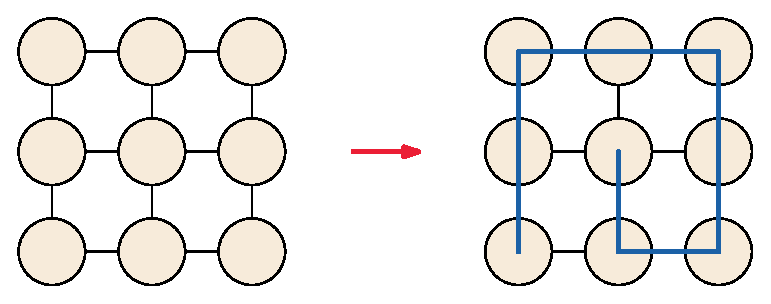
\includegraphics[scale=0.6]{figures/quickfire_north_regional_recursiondepth_01.eps}
\end{center}
% \marginnote[-2\baselineskip]{%
%     \centering
%     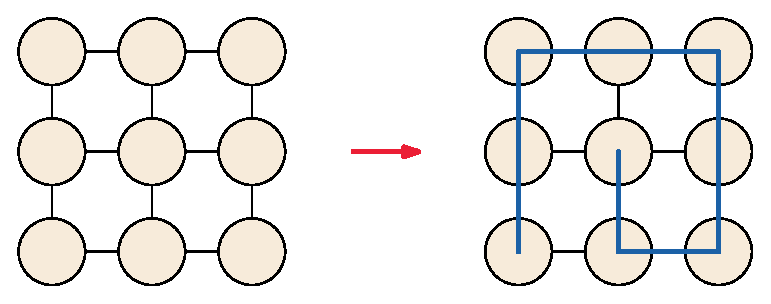
\includegraphics[scale=0.6]{figures/quickfire_north_regional_recursiondepth_01.eps}\\
%     รูปประกอบกรณี\uline{ตัวอย่าง}
% }

\noindent
\textbf{\uline{โจทย์}}\; จงหา Maximum recursion depth ที่เป็นไปได้ 
หากเราสามารถใช้อัลกอริทึม Depth-first search จากโหนดใดก็ได้ในกราฟต่อไปนี้
\begin{center}
    \bigskip
    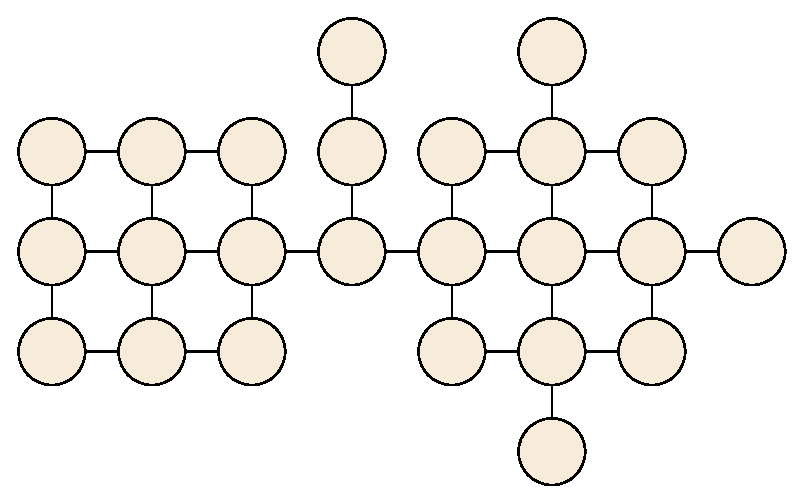
\includegraphics[scale=0.6]{figures/quickfire_north_regional_recursiondepth_02.eps}
\end{center}
